%%
%% SIGGRAPH Asia 2026 Art Papers — blind review submission
%%
\documentclass[sigconf,anonymous]{acmart}

\acmConference[SA '26]{SIGGRAPH Asia 2026}{December 2026}{Tokyo, Japan}

\title{Resonating Distance: Staging Proximity and Closure in a Charity Concert for Ukraine}

\begin{document}

\begin{teaserfigure}
  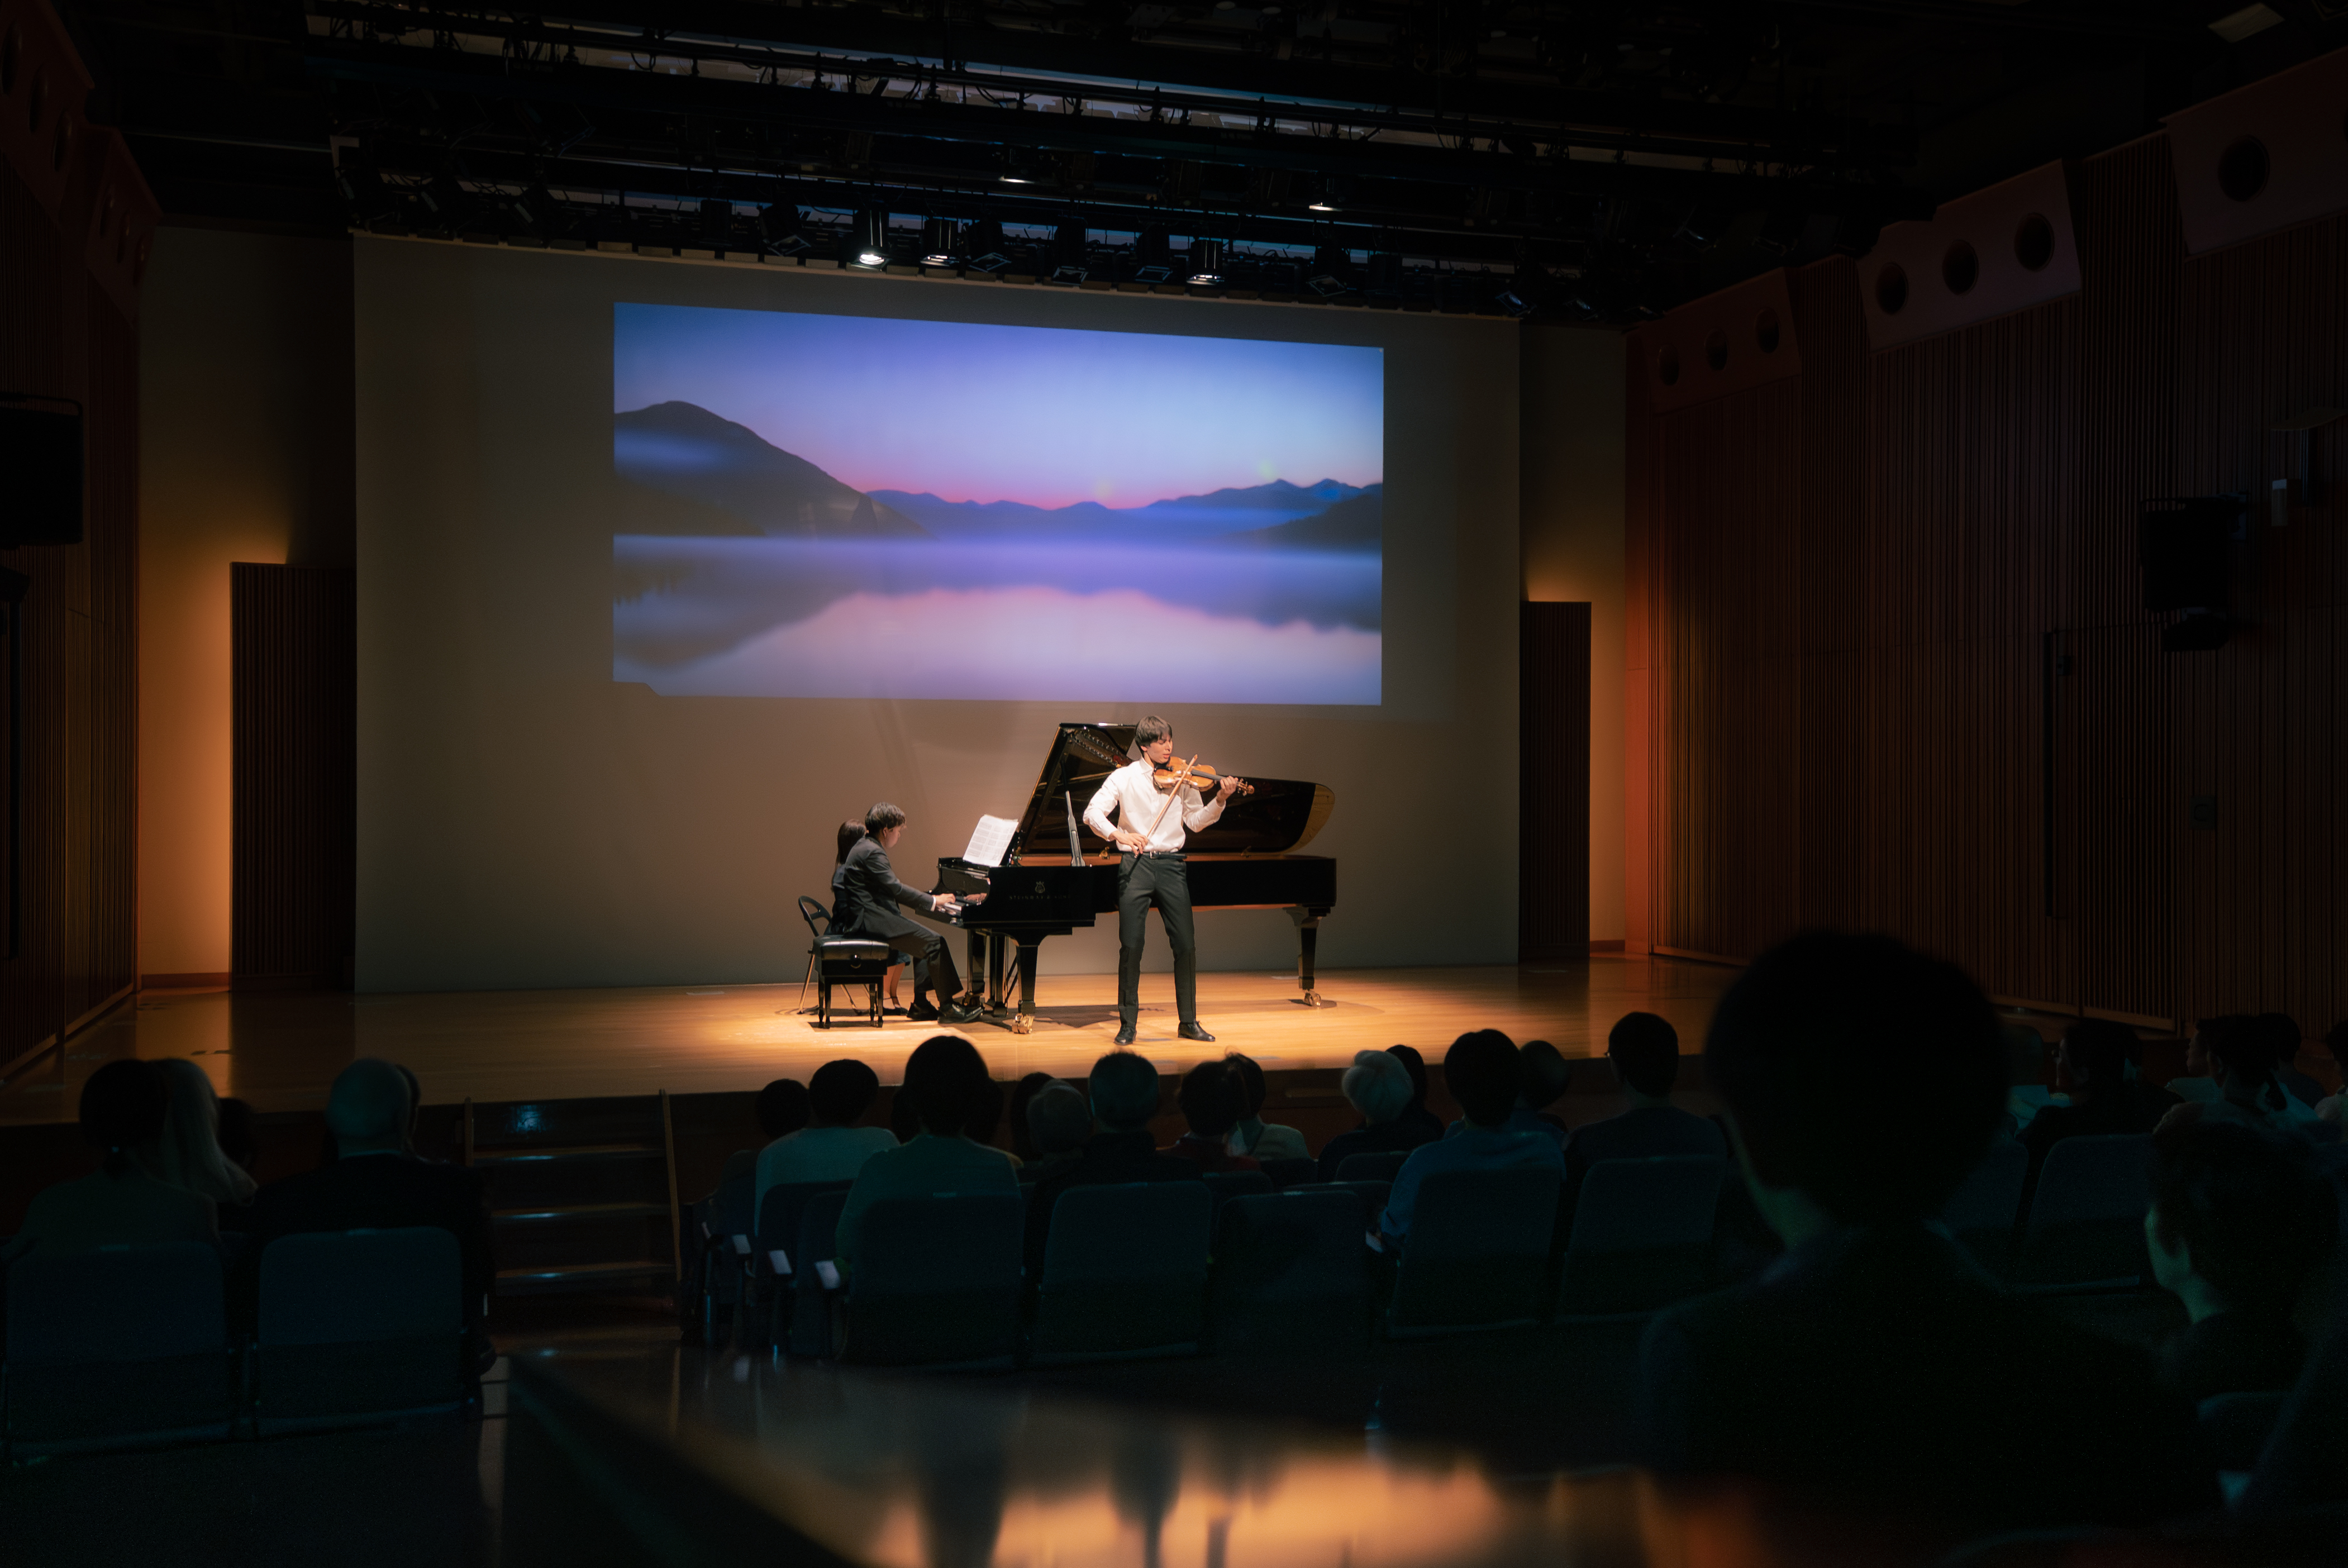
\includegraphics[width=\textwidth]{fig/teaser.jpg}
  \caption{Concert performance at the Tokyo venue (April 2026). The duo performs during
  Movement I (Everyday Life), with a TouchDesigner visual projection showing a serene
  landscape as the digital layer.}
  \label{fig:teaser}
\end{teaserfigure}

\begin{abstract}
We organized a charity classical concert to support children displaced by the Russia-Ukraine
War, connecting venue audiences in Japan with fifteen Ukrainian participants joining remotely.
The design introduced digital elements (video projection, live audience messaging, and remote
participation) within classical concert form, while keeping music as the primary event.
Post-concert surveys and qualitative interviews examined two outcomes: whether the digital
additions displaced the characteristic classical listening experience; and whether the concert
generated sustained engagement with the conflict or primarily the feeling of having engaged.
The music remained the primary experience. The concert converted distance into a
receivable form; the moderation that made the conflict approachable also made it easier
to conclude than to continue.
\end{abstract}

\maketitle

%%
%% Why It Matters
%%
\section*{Why It Matters}

Our goal is to document what charity media art produces, formally and ethically, and to
show that this is a question the SIGGRAPH community should also examine.
Collaborating with classical musicians, reconciling digital technology with a norm-bound
tradition, and designing within a subject as difficult as war: this raises ethical questions
the SIGGRAPH community is positioned to examine but rarely does.

%%
%% 1. Introduction
%%
\section{Introduction}

By 2025, the Russia-Ukraine War had entered its fourth year, and public attention in Japan had
measurably shifted.
Two classical musicians, both from Hiroshima with personal ties to Ukraine, had been
organizing charity concerts for this cause since 2022. They chose to continue despite an
absence of sponsorship, funding this concert through crowdfunding.
This paper documents the charity concert that followed: what it was designed to hold
together, what kind of proximity it produced, and how its own conditions of ethical
moderation shaped the limits of that proximity.

Representing others' suffering through music risks aestheticizing it~\cite{Sontag2003},
but this risk was compounded by the specific conditions these performers faced.
By 2025, audiences with little prior engagement with the Russia-Ukraine War were unlikely
to attend an event framed in political terms; classical music offered a mode of address
that could be entered without prior commitment.
The cost was structural: the more fully the war was rendered as musical experience, the
more it risked becoming a finished object of aesthetic reception rather than a continuing
condition.
Charity practice amplifies this — the emotional response a concert generates can itself
function as completion, substituting for rather than enabling further
action~\cite{Boltanski1999,Chouliaraki2013}.
These are not problems that better technique resolves. They are the conditions under which
this concert was designed.

The classical concert format carries norms that solidified around 1800~\cite{Goehr1992}:
score authority, performer-audience separation, and participation confined to silence and
applause.
These performers are classical musicians who brought their practice to this cause.
Their aspiration was to use the sustained, attentive listening that classical concert demands
as a channel for connection with Ukraine. If audiences could attend to the conflict with
that quality of attention, the resulting proximity might be more than a typical charity
communication produces.
The design challenge is whether additions of this kind can be made to serve that listening
rather than displace it.

Practices integrating digital media into classical performance have been developed by Yoichi
Ochiai in collaboration with the Japan Philharmonic Orchestra~\cite{Ochiai2018,Ochiai2024}.
The present practice used that integration to connect a Japanese audience with a distant
conflict, directing attention toward Ukraine rather than extending the music's expressive
range.

This paper documents a charity classical concert held at two venues in Japan in 2026, with
fifteen Ukrainian participants joining remotely.
Drawing on 118 audience messages, a post-concert survey ($n=14$), and qualitative interviews
($n=10$), we report what the concert produced in two registers: whether digital media
interpolated into a classical format can sustain its characteristic listening experience, and
whether a charity concert of this kind generates engagement with a distant conflict or
primarily provides the feeling of having engaged.
The music remained the primary experience. The concert converted distance into a receivable
form; the moderation that made the conflict approachable also structured the experience
toward completion rather than continued engagement.

%%
%% 2. Practice Context
%%
\section{Practice Context}

Two of the authors, classical musicians based in western Japan with personal ties to Ukraine,
began organizing charity concerts in response to the Russia-Ukraine War in 2022.
Over the following three years they performed more than twenty concerts across Japan and
the United States, donating proceeds to organizations supporting civilians affected by the
conflict.

By 2025, the war had entered its fourth year and public engagement in Japan had measurably
declined.
The organizing team approached approximately twenty corporate sponsors for the 2026 concert;
no agreements were reached.
Organizers were told that the cause no longer carried sufficient public profile for corporate
investment, among other reasons.
Venue staff cautioned that a standard classical concert on this subject would struggle to
draw an audience.
These obstacles converged on a single design question: how to reach audiences with little
prior engagement with the Russia-Ukraine War and, consequently, few existing reasons to attend.
The goal was for Ukrainian voices to reach Japanese audiences and for that connection to
produce concrete support through a donation channel linked to a partner organization
supporting civilians, in particular children, affected by the Russia-Ukraine War.
Whether that chain from attention to action was reliable is what this paper examines.
Crowdfunding replaced corporate sponsorship and the concert proceeded.

%%
%% 3. Concert Design
%%
\section{Concert Design}

\subsection{Design Requirements}

The concert was designed to avoid attributing collective culpability to any nation or people,
to foreground civilian experience over political framing, to involve Ukrainian participants
in shaping the content, and to direct proceeds to a partner organization with identifiable
beneficiaries.

On the performance side, the musical programme remained the primary event.
Technical elements were kept subordinate to the score's expressive intentions.
Submitted audience messages were reviewed for appropriateness before display; none were excluded.

\subsection{Design Process and Decision-Making}

The concert design was developed over several months by two performing musicians, a video
artist, and a technical producer.
The performing musicians held final authority over artistic decisions, with the other two
contributing within those decisions.
Rotary Club Dnipro City (Ukraine) was consulted throughout on questions of representational
appropriateness, including whether specific imagery or framing would be received as
respectful by Ukrainian audiences.

The team's central question was how to use digital elements to bring the reality of the
Russia-Ukraine War closer to audiences, without disrupting the musical experience the
classical format depends on.

\subsection{Three-Part Dramaturgy}

\begin{table*}
\caption{Concert programme with scoring and compositional intent by movement.}
\label{tab:programme}
\small
\begin{tabular}{llp{5.5cm}p{5.5cm}}
\toprule
Mv. & Piece & Scoring & Intent \\
\midrule
\multicolumn{4}{l}{\textbf{I. Everyday Life}} \\
 & Bach: Cello Suite No.~3, Bourrées I\&II, Gigue & Viola solo & Pre-war daily life; ordered beginning \\
 & Schubert: Arpeggione Sonata & Duo & Peaceful coexistence as dialogue \\
 & Schumann: Von fremden Ländern (Kinderszenen) & Piano solo & Children's perspective; homage to Ukrainian children \\
 & Kreisler: Liebesleid & Duo & Love and pathos; premonition within happiness \\
\midrule
\multicolumn{4}{l}{\textbf{II. Sudden Tragedy}} \\
 & Rachmaninoff: The Bells Prelude & Piano solo & Alarm; premonition of loss \\
 & Penderecki: Cadenza & Viola solo & Dissonance as direct expression of war \\
 & Rachmaninoff: Moments Musicaux No.~4 & Piano solo & Passion and silence; stupor after destruction \\
 & Live connection with Ukraine & Video & Reality break; confronting the present \\
\midrule
\multicolumn{4}{l}{\textbf{III. Rebirth and Prayer}} \\
 & Kreisler: Praeludium and Allegro & Duo & Powerful revival; two voices reunited \\
 & Kreisler: Tambourin Chinois & Duo & Recovery of vitality \\
 & Sakamoto: Energy Flow & Piano solo & Quiet healing toward rebirth \\
 & Massenet: M\'{e}ditation (Tha\"{i}s) & Duo & Prayer; transcendence; close of concert \\
\midrule
\multicolumn{4}{l}{\textit{Encore}} \\
 & Monti: Cs\'{a}rd\'{a}s & Duo & Joy of living; heat to take home \\
\bottomrule
\end{tabular}
\end{table*}

The concert moved through three phases of experience under conflict (Table~\ref{tab:programme}),
and that structure governed the musical programme, visual projection, and message framing
throughout.

\subsubsection{Digital Media}

Visual projection was developed in TouchDesigner through discussion between the performing
musicians and the video artist, beginning from the musical programme.
Movements one and three, anchored in realist emotional territory, received imagery drawn
from Ukrainian civilian life.
Movement two, representing sudden tragedy, received abstract visual treatment to avoid
both the shock of documentary footage and the sentimentality of direct representation
(Figure~\ref{fig:warimage}).
The video artist refined the work through four rounds of feedback with the lead violinist
before the programme was fixed.

\begin{figure}[h]
  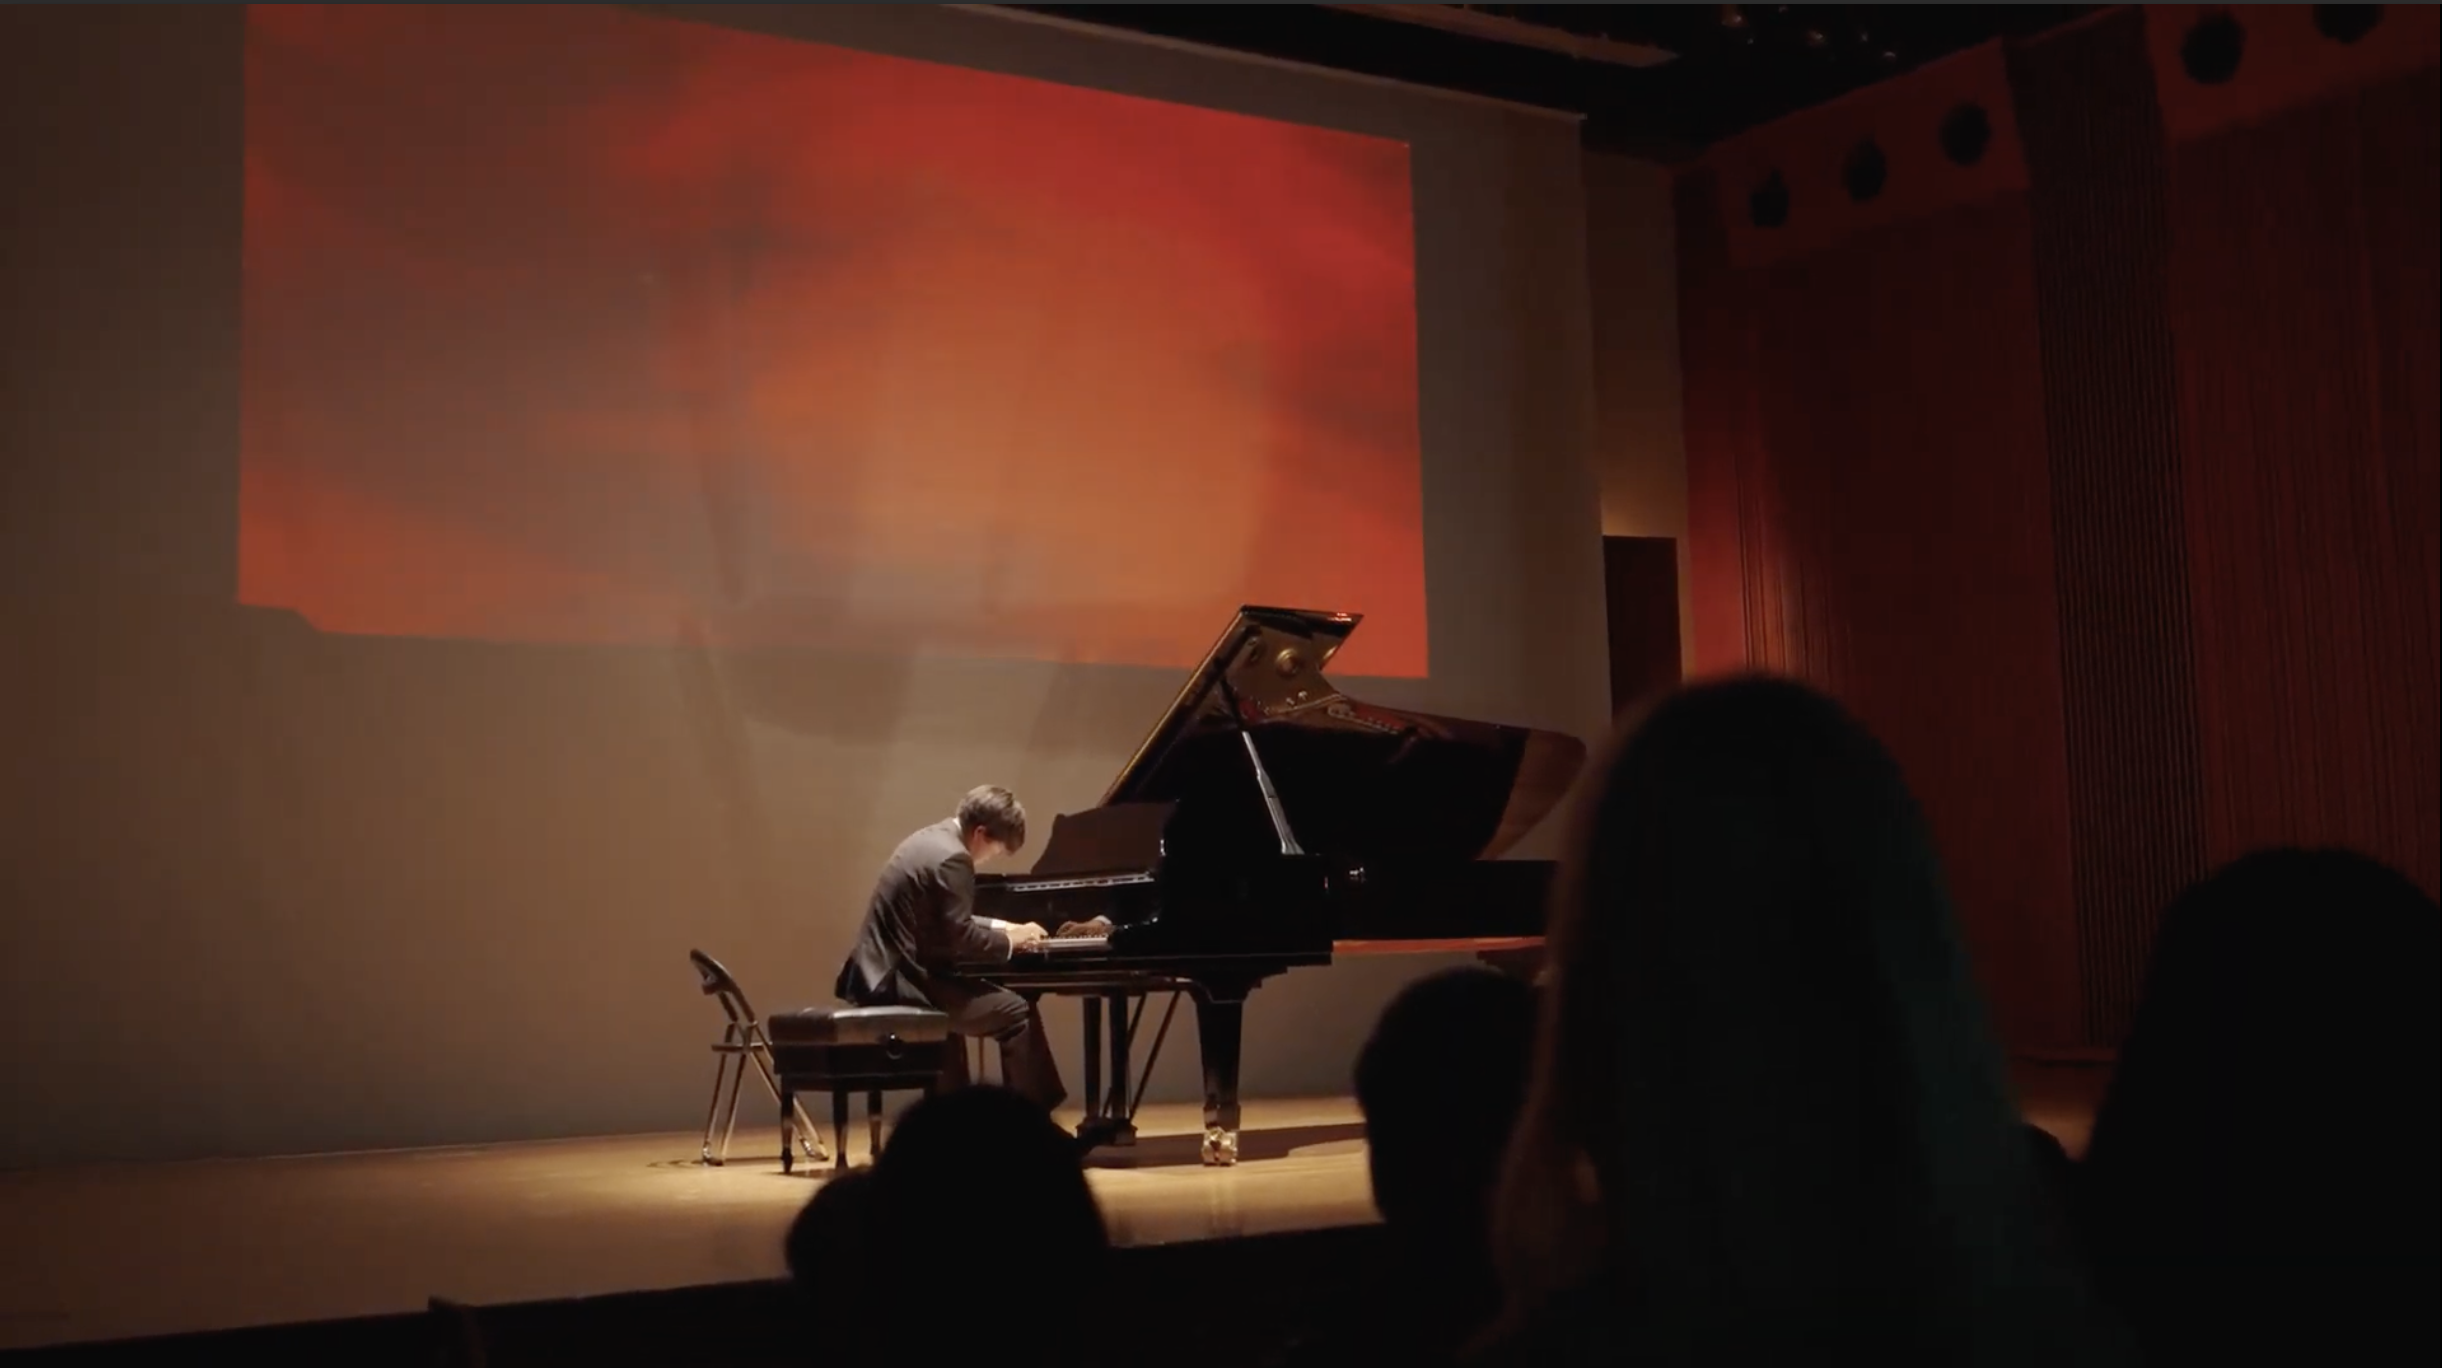
\includegraphics[width=\columnwidth]{fig/War Image FIgure.png}
  \caption{Abstract visual projection during Movement II (Sudden Tragedy), rendered in
  TouchDesigner. The red-orange treatment avoids documentary realism while maintaining
  emotional register.}
  \label{fig:warimage}
\end{figure}

\subsubsection{Audience Interaction}

A web-based messaging system allowed venue attendees and Ukrainian participants to submit
short messages during the concert.
Before display, submitted messages were reviewed to confirm that none were inappropriate;
no messages were excluded.
The full set of submissions was displayed on stage during the encore, when Japanese
and Ukrainian voices appeared together as the concert concluded
(Figure~\ref{fig:message}).

\begin{figure}[h]
  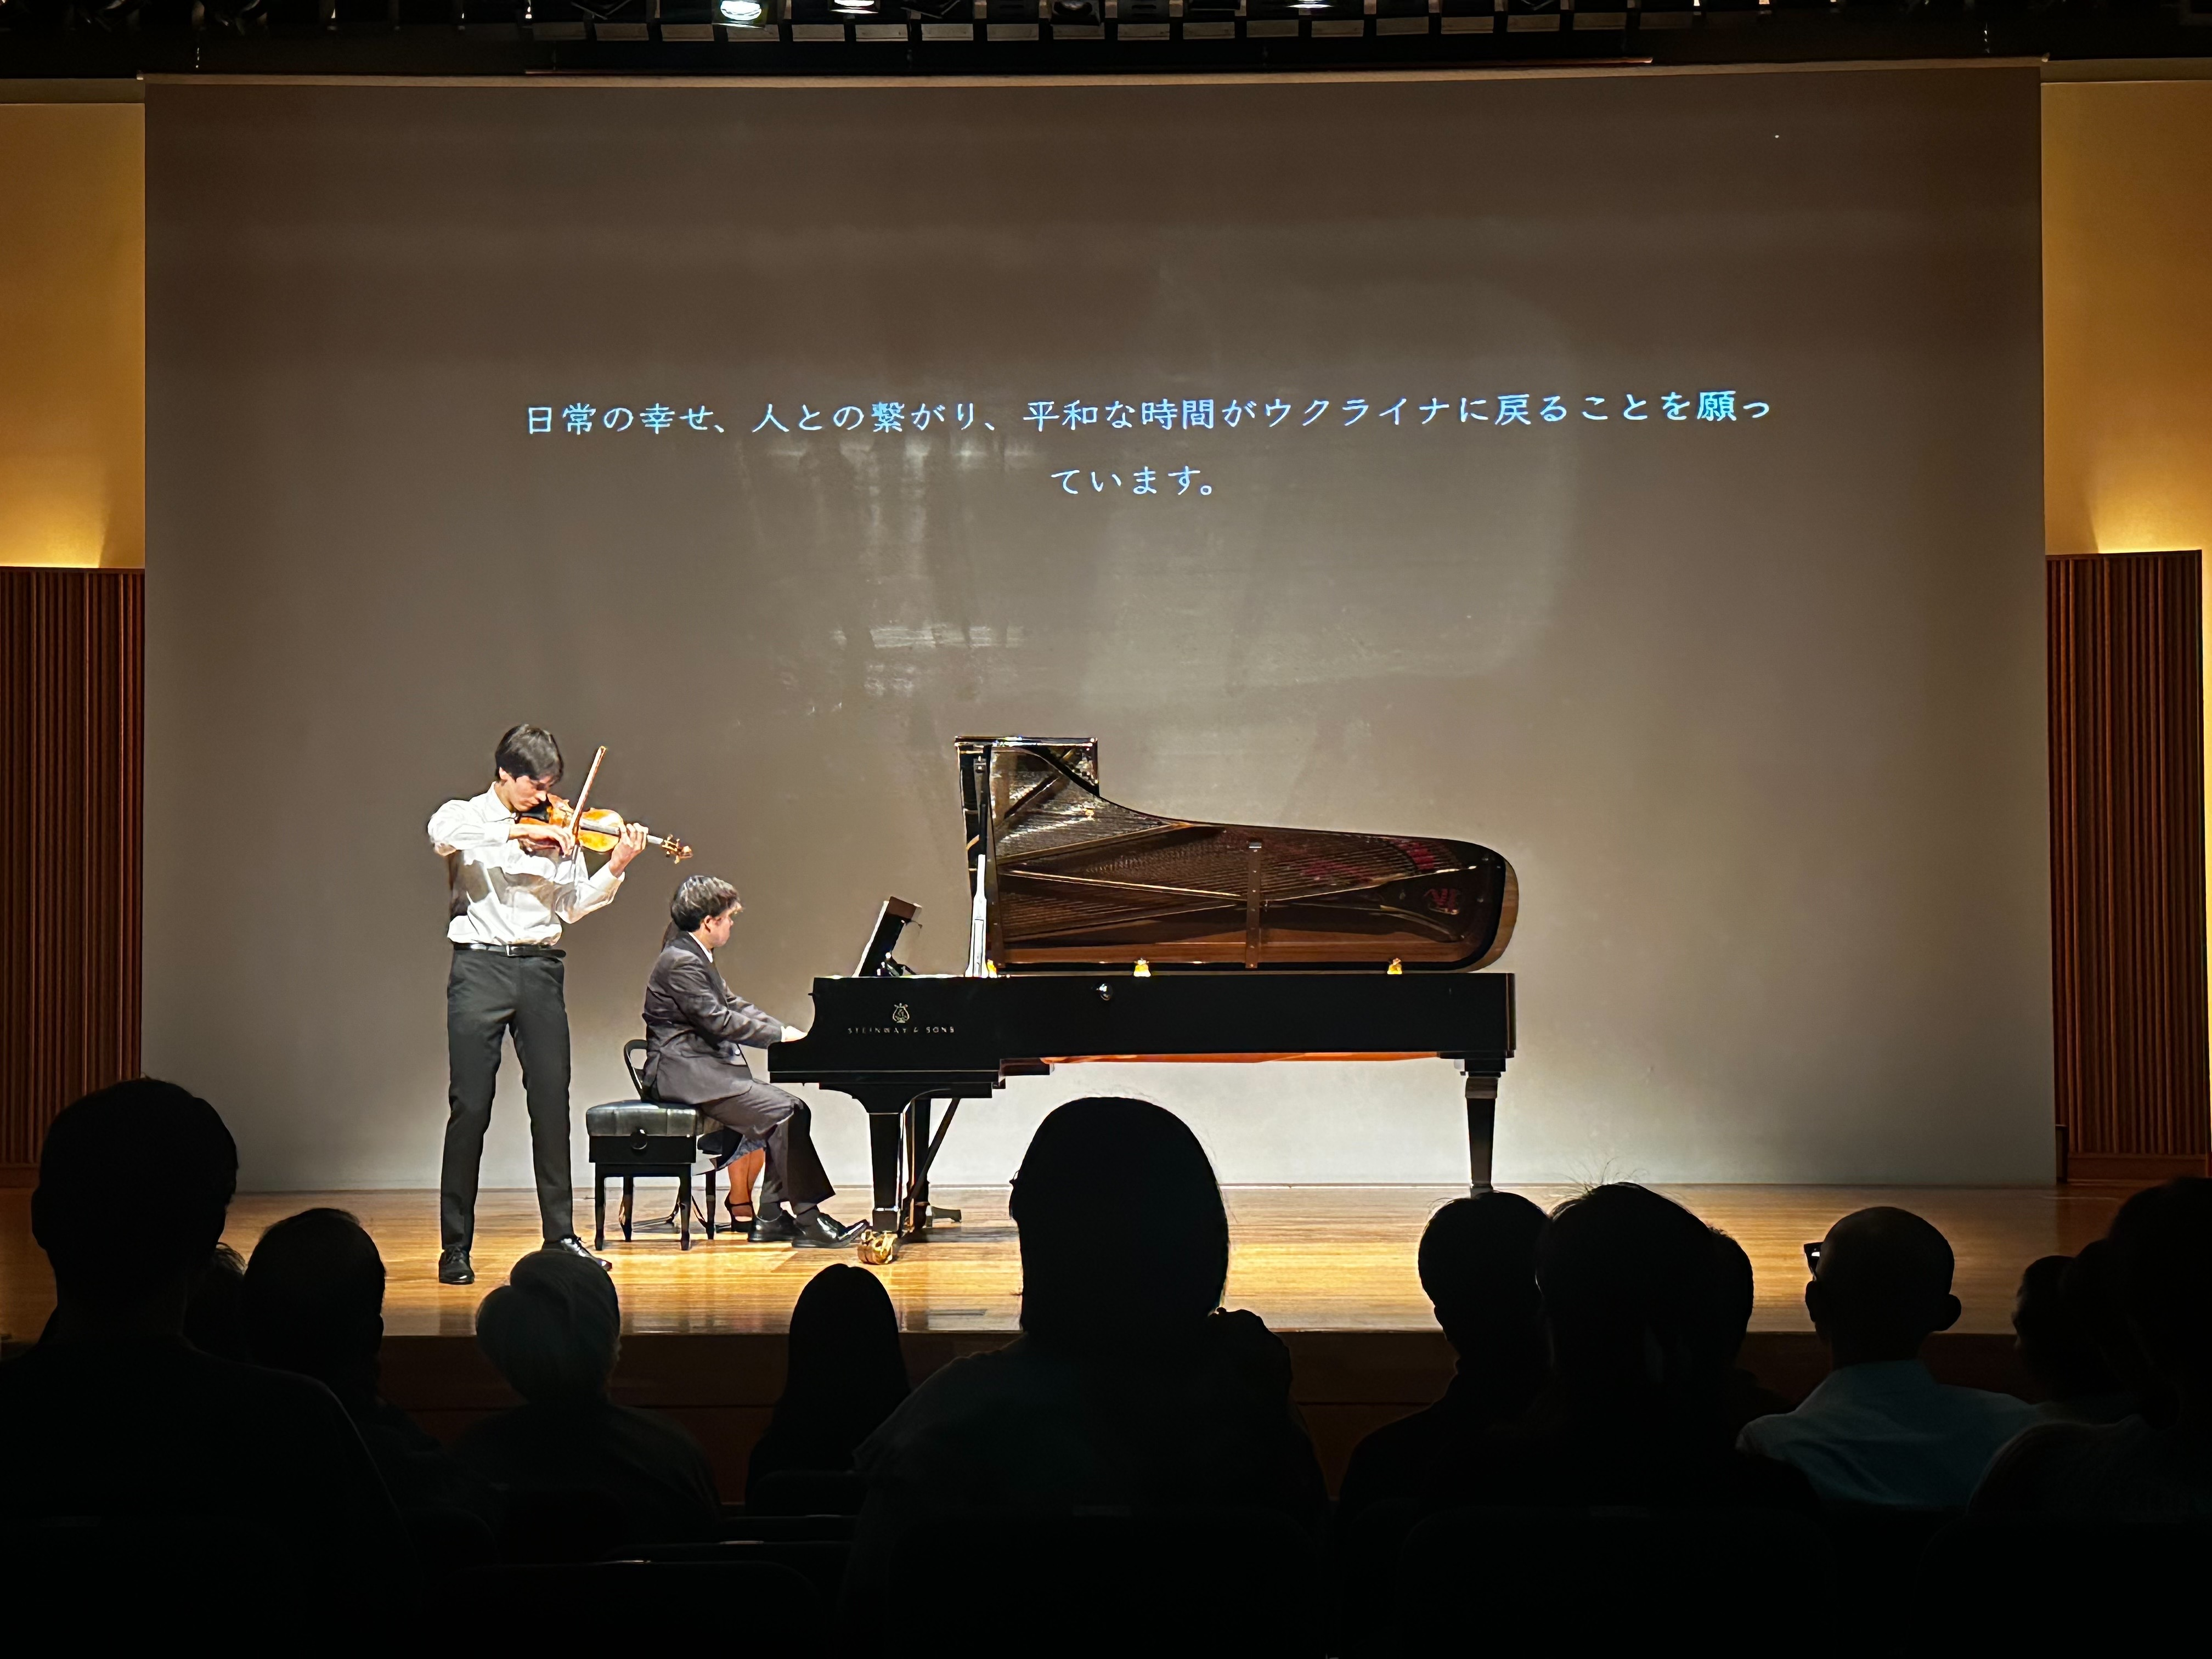
\includegraphics[width=\columnwidth]{fig/A_Message_Comming_From_Audience.jpg}
  \caption{An audience message displayed on stage during the encore. The text reads:
  ``I pray that everyday happiness, human connection, and peaceful times will return to
  Ukraine.'' Submissions from venue attendees and Ukrainian participants were reviewed
  before display; none were excluded.}
  \label{fig:message}
\end{figure}

\subsubsection{Remote Connection with Ukraine}

Ukrainian participants joined the concert via a video conferencing platform routed through
the venue's sound infrastructure.
The connection was configured for access from Ukraine, where standard consumer platforms
faced intermittent restrictions during the conflict period.
Participants could observe the live performance and submit messages through the same
system as venue attendees.
This arrangement made the boundary between live and remote presence a practical design
constraint rather than a categorical distinction~\cite{Auslander2008}.

%%
%% 4. Study and Materials
%%
\section{Study and Materials}

\subsection{Concert Overview}

The concert was held at two venues: Tokyo (April 2026, 153 attendees) and Hiroshima
(May 2026, 156 attendees).
Fifteen participants joined from Ukraine remotely.
Proceeds were directed to Rotary Club Dnipro City, which supports children affected by the
Russia-Ukraine War, including through music education programs.
Both performances concluded without production incidents.

\subsection{Audience Messages}

\begin{figure*}
  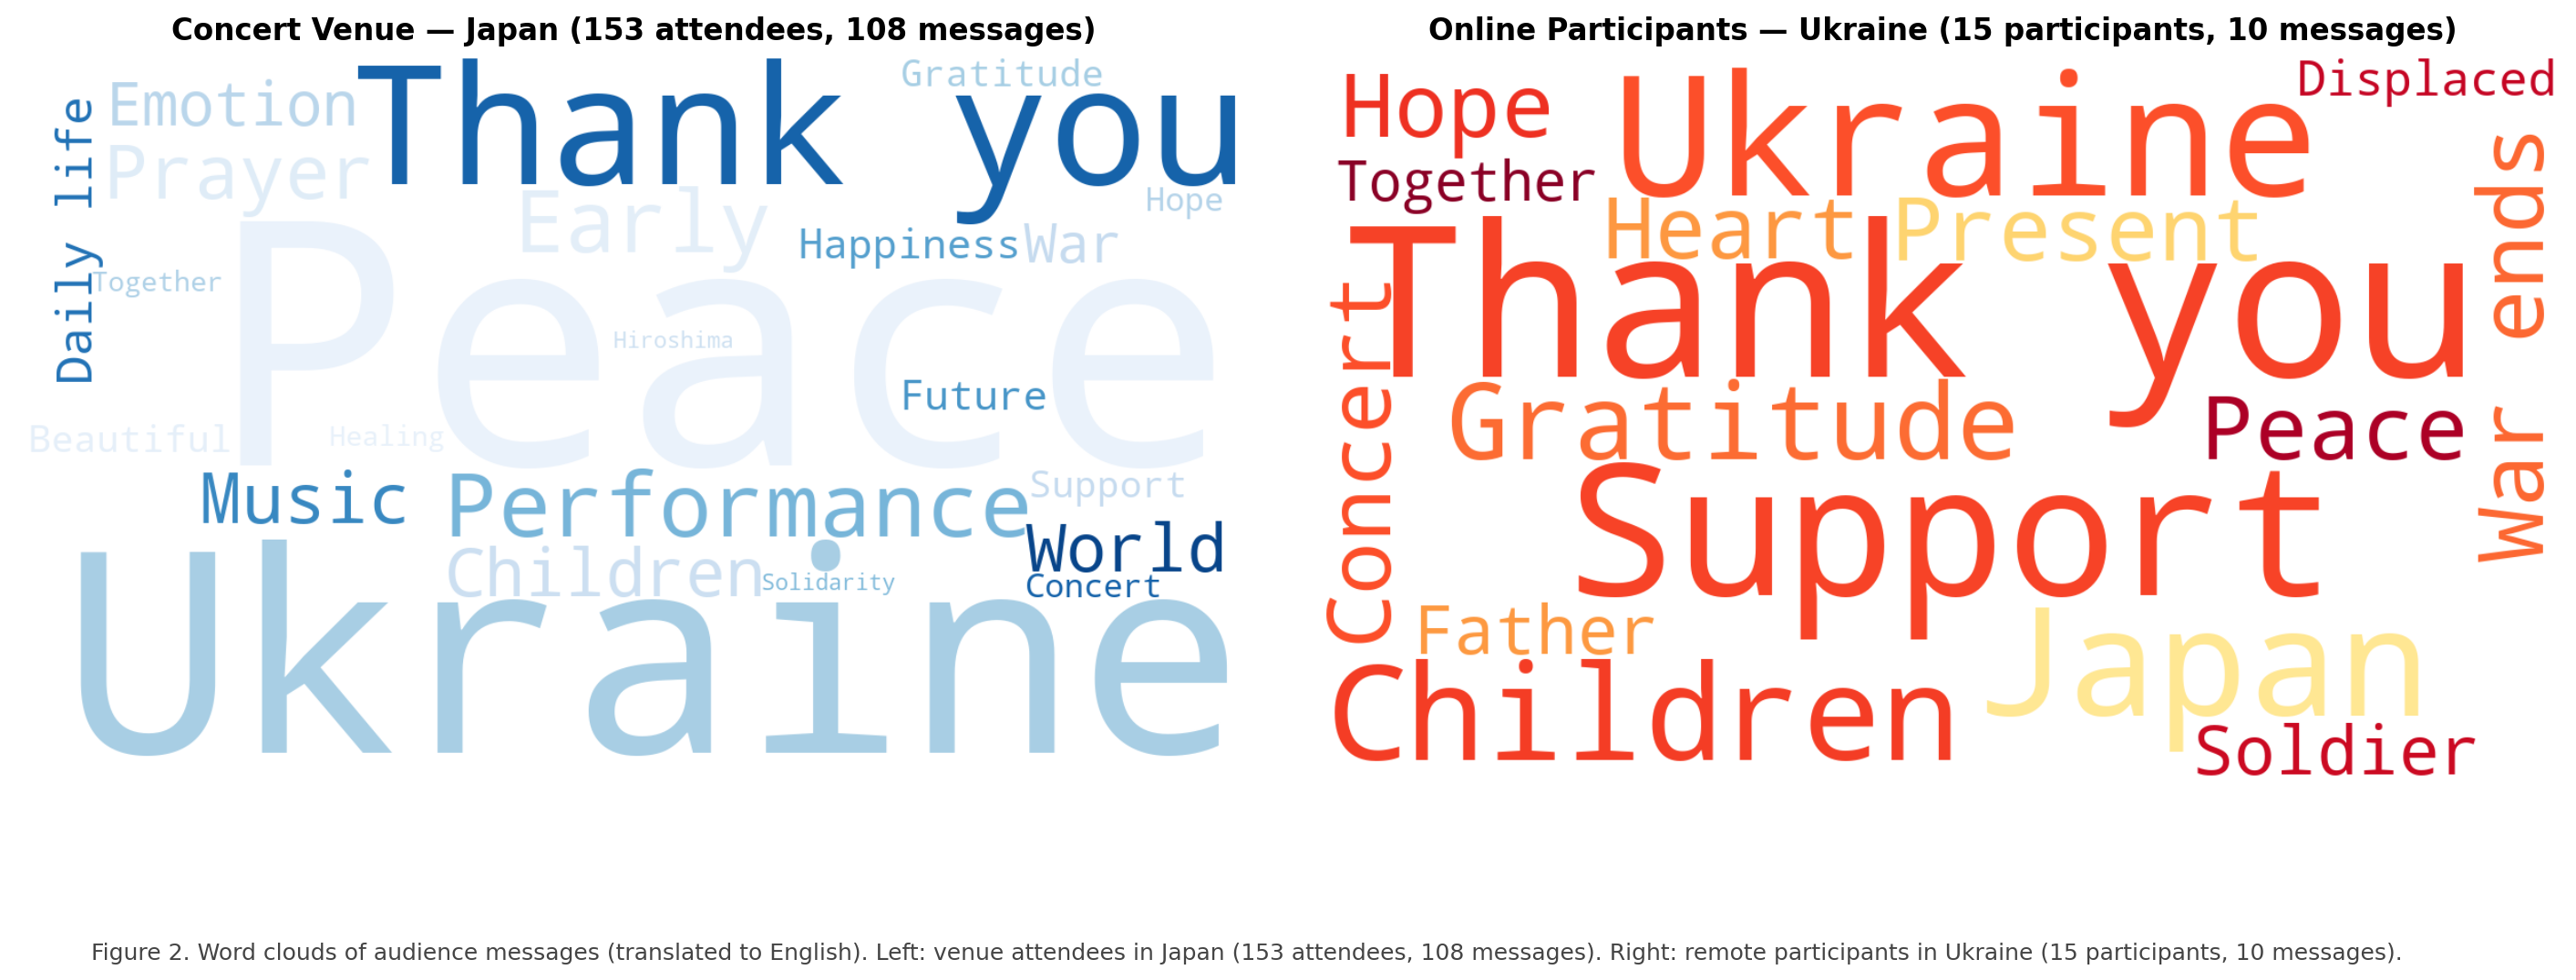
\includegraphics[width=\textwidth]{figure2_wordclouds.png}
  \caption{Word clouds of audience messages translated to English.
  Left: Japan (153 attendees, 108 messages).
  Right: Ukraine (15 participants, 10 messages).}
  \label{fig:wordclouds}
\end{figure*}

Of 118 messages collected (108 from venue attendees and 10 Ukrainian submissions), the most frequent terms in venue messages were Peace (37),
Ukraine (26), Thank you (25), Performance (23), and Prayer (17), clustering around
abstract hope and gratitude.
Ukrainian participant messages occupied a different register: thanks to Japan were
accompanied by references to concrete circumstances (``my father is in the military,''
``support for displaced children'').
Figure~\ref{fig:wordclouds} renders both sets as word clouds.
This asymmetry is analyzed in Section~5.2.

\subsection{Post-Concert Survey and Interviews}

A post-event survey was distributed by email; 14 responses were received.
Ten respondents subsequently participated in qualitative interviews examining post-concert
behavior and subjective experience.
The survey asked about the sense of proximity to the Russia-Ukraine War produced by the
concert, the character of that proximity, the kind of experience the concert resembled, and
whether it felt like an entry point or a conclusion.
Interviews with Ukrainian participants were coordinated through the Dnipro Rotary Club;
specific interview excerpts will be incorporated in the final version of this paper.

%%
%% 5. Findings and Discussion
%%
\section{Findings and Discussion}

\subsection{Media Design as Interpolation of Classical Listening}

Survey respondents classified the primary character of their concert experience as music
listening more frequently than any other category, ahead of ``time to think about
Ukraine,'' ``prayer or memorial,'' or ``charity participation.''
This is consistent with the classical listening frame remaining primary, though survey
categorization alone does not establish it.
The more direct evidence comes from qualitative interviews: participants who attended
primarily for the music described their experience in musical terms first, treating digital
elements as context rather than as the primary object of attention.

The mechanism described in interviews was one of supplementary completion.
Music was reported to evoke scenes indirectly rather than transmit images directly.
Civilian-focused imagery --- photographs of everyday life and children's faces --- provided
visual fragments through which participants without prior knowledge of Ukraine could
organize and reconstruct the scene the music suggested.
Interviewees noted that this felt less coercive than verbal or explicit political framing,
and differed from their prior encounters with images of the war.
Within Goehr's framework~\cite{Goehr1992}, the music retained its authority over the
event's expressive logic; digital elements operated in its service rather than displacing it.

The interpolation held at the level of overall framing, but specific failures were
identified.
Moving imagery competed with auditory attention for several interviewees, shifting focus
from the music to the visual.
Sustained projection without variation produced fatigue; several interviewees noted
wanting more variation in the density of digital presence across the programme.
Abrupt introduction of digital content within classical concert form caused disorientation.
Mismatches between the realism level of imagery and the listener's prior contextual
knowledge compounded these difficulties: participants without existing mental images of
Ukraine found some visual material difficult to integrate with the musical content.
The density of digital presence, the realism level of imagery, and the pacing of
transitions each require calibration against the audience's existing context knowledge,
specifying what successful interpolation demands rather than refuting its feasibility.

\subsection{Proximity as Closure}

The character of the proximity the concert produced is visible in what audiences wrote.
Japanese venue messages clustered around abstract and ritual vocabulary: peace, prayer,
gratitude, performance.
Ukrainian participant messages occupied a different register: gratitude to Japan appeared
alongside references to specific circumstances --- a father in the military, displaced
children, concrete support needs.
The asymmetry reflects not indifference but the structure of the gap the concert was
designed to bridge.
For Japanese audiences, Ukraine arrived as a form that was emotionally shareable; for
Ukrainian participants, Japan remained a context of aesthetic norms within which to
express concrete conditions.

What the concert produced was not a reduction of distance but a conversion of
it~\cite{Heidegger1971}.
Distance was rendered into a form --- musical, prayerful, formally contained --- that
Japanese audiences could receive and share.
The same moderation that made the conflict approachable also made it easier to complete
as an experience.
Of ten interviewees, only one sought further information about the Russia-Ukraine War
after the concert.
The emotional response appears to have functioned as its own completion, consistent with
the structural tendency Boltanski and Chouliaraki describe: emotional engagement
substituting for rather than enabling further
action~\cite{Boltanski1999,Chouliaraki2013}.
This tendency was not a correctable design error; it follows from the form.

This paper analyzes this not as failure but as the structural condition of charity media
practice.
One survey respondent described the concert as ``both an entry point and a conclusion.''
The design terms that made participation feel meaningful --- attentive listening, restrained
imagery, a shared message channel --- were the same terms that allowed it to feel
complete~\cite{Bishop2004}.
Whether smooth reception indicates successful communication or comfortable
consumption~\cite{Sontag2003} cannot be resolved from this data; the low rate of
follow-through is consistent with both interpretations.

\subsection{Implications for Practice}

For practitioners designing digital mediation within classical form, three variables emerge
as requiring explicit calibration: the realism level of visual content relative to the
audience's prior knowledge of the subject; the density and distribution of digital presence
across the programme; and the pacing of transitions between digital-intensive and
classical-only passages.
The same design produced different experiences for audiences with and without prior
engagement with the subject, suggesting that supplementary framing (such as programme notes or a brief orientation)
may be necessary for audiences with no prior exposure.

For practitioners working at the intersection of charity and war, the more fundamental
question is not what the emotional resonance produces but what the conversion required
to produce it costs.
The vocabulary asymmetry documented here --- Japanese audiences receiving Ukraine as
peace and prayer, Ukrainian participants expressing family, military, and displacement ---
indicates that the concert achieved proximity at the price of abstraction.
The gap between that abstraction and sustained engagement remains an open question for
future practice.

%%
%% 6. Conclusion
%%
\section{Conclusion}

Digital interpolation into classical performance is possible but requires calibration of
three variables against the audience's existing context knowledge, as examined in
Section~5.1.
The more persistent challenge lies in what Section~5.2 documents: a charity concert does
not simply bring distant suffering closer; it converts distance into a form that is
emotionally receivable and formally complete, and that conversion is not a design failure
to be corrected but a structural condition to be named.
Future practice begins with the harder question: not how to avoid the conversion, but
whether it can be held visible --- designing with honesty about what the concert produces
alongside what it aspires to produce.

%%
%% References
%%
\bibliographystyle{ACM-Reference-Format}
\bibliography{references}

\end{document}
